\documentclass{beamer}

\usepackage[utf8]{inputenc}
\usetheme{default}

\usepackage{listings}
\lstset{
basicstyle=\small\ttfamily,
columns=flexible,
breaklines=true
}
\usepackage{enumerate}
\usepackage{epstopdf}
\usepackage{multicol}
\usepackage{amsmath}
\usepackage{tikz}
\usepackage{mathdots}
\usepackage{yhmath}
\makeatletter
\DeclareMathSizes{\f@size}{10}{7}{7}
\makeatother

\title[66.20/86.37]{U.B.A. - Facultad de Ingeniería\\\vspace{0.25cm} 66.20/86.37 Organización de Computadoras
\\Desempeño}
\author{Práctica}
\date{1$^{er}$ cuatrimestre 2020}


\begin{document}
\begin{frame}
\titlepage % Print the title page as the first frame
\end{frame}

\begin{frame}
\frametitle{Desempeño}
Medir la performance en forma precisa y correcta para comparar distintas computadoras es crítica para los compradores y por lo tanto para los diseñadores.

\bigskip
Para maximizar la performance vamos a querer minimizar el tiempo de respuesta o el tiempo de ejecución de una determinada tarea. Con lo cual, podemos relacionar la performance y el tiempo de ejecución para una computadora X.

\[ \text{Performance}_\text{x} = \frac{1}{\text{Tiempo de ejecución}_\text{x}} \]
\end{frame}

\begin{frame}
\frametitle{Desempeño}
Si la performance de X es mayor que la performance de Y, tenemos que:

\[ \text{Performance}_\text{x} > \text{Performance}_\text{y} \]
\[ \frac{1}{\text{Tiempo de ejecución}_\text{x}} > \frac{1}{\text{Tiempo de ejecución}_\text{y}} \]
\[ \text{Tiempo de ejecución}_\text{y} > \text{Tiempo de ejecución}_\text{x} \]

\bigskip
El tiempo de ejecución de Y es mayor que el de X, es decir, X es más rápida que Y.

\end{frame}

\begin{frame}
\frametitle{Benchmarks}
\begin{itemize}
\item kernels, partes pequeñas y significativas de una aplicación real.
\item programas de juguete, son programas de no más de 100 líneas, como el quicksort.
\item benchmarks sintéticos, son programas inventados que aprovechan ciertas características de una determinada computadora, como Dhrystone.
\end{itemize}
\end{frame}

\begin{frame}
\frametitle{Ley de Amdahl}
La ley de Amdahl define el speedup que puede ser obtenido al utilizar una mejora particular. 

\bigskip
El speedup está determinado por la relación:

\tiny
\[\text{speedup} = \frac{\text{Performance de toda la tarea utilizando la mejora cuando es posible}}{\text{Performance de toda la tarea sin ninguna mejora}} \]

\bigskip
\normalsize
O de otro modo,

\tiny
\[\text{speedup} = \frac{\text{Tiempo de ejecución de toda la tarea sin utilizar la mejora}}{\text{Tiempo de ejecución de toda la tarea utilizando la mejora cuando es posible}} \]

\end{frame}

\begin{frame}
\frametitle{Ley de Amdahl}
La ley de Amdahl entonces nos brinda una forma rápida de encontrar el speedup de una mejora que depende de dos factores:

\begin{enumerate}
 \item La fracción de tiempo del tiempo original que se puede aplicar una mejora.
 \item La mejora obtenida al aplicar el nuevo modo, esto es, que tan rápido correrá el sistema si se aplica la mejora.
\end{enumerate}

\bigskip
\tiny
$
\text{Tiempo de ejecución}_\text{nuevo} = \text{Tiempo de ejecución}_\text{viejo}  \times \left( (1 -  \text{Fraccion}_\text{mejorable} + \frac{\text{Fraccion}_\text{mejorable}}{\text{speedup}_\text{local}} \right)
$

\end{frame}

\begin{frame}
\frametitle{Ecuación de desempeño del CPU}
\[ \text{CPU time} = \text{Instruction count} \times \text{CPI} \times \text{Clock cycle time} \]

\[ \text{CPU time} = \frac{\text{Instruction count} \times \text{CPI}}{ \text{Clock rate}} \]

\tiny
\begin{table}[h!]
\centering
\begin{tabular}{|l|l|}
\hline
   
\textbf{Componente de performance} & \textbf{Unidad de medida}  \\ \hline
Tiempo de ejecución de CPU para un programa & Segundos por programa \\ \hline
Instruction count (Cantidad de instrucciones) & Instrucciones ejecutadas por el programa \\ \hline
Ciclos de reloj por instrucción (CPI) & Promedio de ciclos de reloj por instrucción \\ \hline
Tiempo de ciclo de reloj (Clock cycle time) & Segundos por ciclo de reloj \\ \hline
\end{tabular}
\end{table}

\[ \text{Time} = \frac{\text{Seconds}}{\text{Program}}= \frac{\text{Instructions}}{\text{Program}} \times \frac{\text{Clock Cycles}}{\text{Instruction}} \times \frac{\text{Seconds}}{\text{Clock Cycles}} \]


\end{frame}

\begin{frame}
\frametitle{Medición de desempeño}

\begin{itemize}
\item CPU execution time o CPU time. El tiempo total que toma la CPU en computar una tarea específica.
\item user CPU time. El tiempo de CPU que toma el programa en sí.
\item system CPU time. El tiempo de CPU que toma el sistema operativo realizando tareas para el programa.
\end{itemize}

\bigskip
Una alternativa a medir tiempo es MIPS (millones de instrucciones por segundo). Para un dado programa, MIPS se calcula:

\[ \text{MIPS} = \frac{\text{Intruction count}}{\text{Execution time} \times 10^6} \]  

\end{frame}


\begin{frame}
\frametitle{Ejercicio 1.2 CAAQA 3ed}
In this exercise, assume that we are considering enhanc- ing a machine by adding vector hardware to it. When a computation is run in vec- tor mode on the vector hardware, it is 10 times faster than the normal mode of execution. We call the percentage of time that could be spent using vector mode the percentage of vectorization.Vectors are discussed in Appendix G, but you don’t need to know anything about how they work to answer this question!
\end{frame}

\begin{frame}
\frametitle{Ejercicio 1.2 CAAQA 3ed}
\begin{enumerate}[a.]
\item Draw a graph that plots the speedup as a percentage of the compu- tation performed in vector mode. Label the y-axis “Net speedup” and label the x-axis “Percent vectorization.”
\item What percentage of vectorization is needed to achieve a speedup of 2?
\item What percentage of the computation run time is spent in vector mode if a speedup of 2 is achieved?
\end{enumerate}
\end{frame}

\begin{frame}
\frametitle{Ejercicio 1.2 CAAQA 3ed}
\begin{enumerate}[a.]\setcounter{enumi}{3}
\item What percentage of vectorization is needed to achieve one-half the maximum speedup attainable from using vector mode?
\item Suppose you have measured the percentage of vectorization for programs to be 70\%. The hardware design group says they can double the speed of the vector hardware with a significant additional engineering investment. You wonder whether the compiler crew could increase the use of vector mode as another approach to increasing performance. How much of an increase in the percentage of vectorization (relative to current usage) would you need to obtain the same performance gain as doubling vector hardware speed? Which investment would you recommend?
\end{enumerate}
\end{frame}

\begin{frame}
\frametitle{Ejercicio 1.2 CAAQA 3ed - Resolución}
\begin{enumerate}[a.]
\item
\end{enumerate}
Partiendo de la Ley de Amdahl, así como los datos del enunciado, tenemos que $ SU_g = \frac{1}{(1-f) + \frac{f}{10}} = \frac{1}{1 - 0,9 \times f}$
 Sabemos también que $ f \in [0, 1] $. Podemos calcular el valor de $SU$ en los extremos:
 
\bigskip
 \begin{itemize}
 \item Si no es posible aplicar la mejora, $f = 0 \implies SU_g = 1$
 \item Si la mejora es aplicable a todo el tiempo de ejecución, $ f = 1 \implies SU_g = SU_L = 10 $
 \end{itemize}
\end{frame}

\begin{frame}
\frametitle{Ejercicio 1.2 CAAQA 3ed - Resolución}

 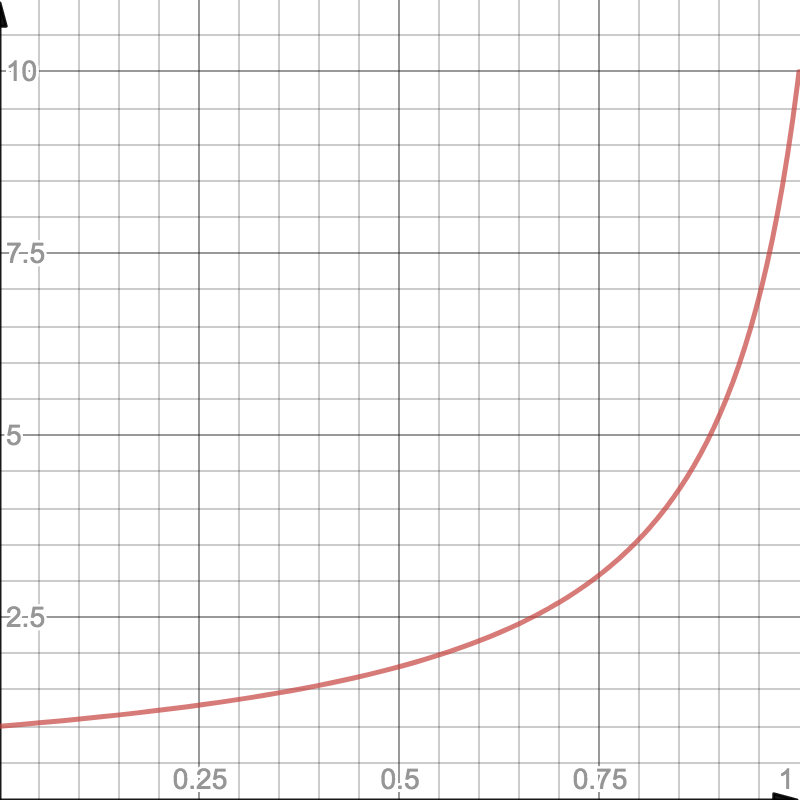
\includegraphics[scale=0.25]{amdahl_resuelto_1.png}

\end{frame}

\begin{frame}
\frametitle{Ejercicio 1.2 CAAQA 3ed - Resolución}
\begin{enumerate}[b.]
\item
\end{enumerate}
¿Qué porcentaje de vectorización es necesaria para alcanzar un $SU$ global de 2?

 Utilizando la ley de Amdahl podemos despejar $f$

 $$ 2 = \frac{1}{1 - 0,9 \times f}$$
 $$ f  = \frac{5}{9} $$

\end{frame}


\begin{frame}
\frametitle{Ejercicio 1.2 CAAQA 3ed - Resolución}
\begin{enumerate}[c.]
\item
\end{enumerate}

Partiendo de la definición de $SU$, tenemos que 

 $$ SU_g = \frac{T_O}{T_N} = 2 \implies f = \frac{5}{9} $$

 $$ SU_L = \frac{T_m}{T'_m} = 10,\quad siendo \quad T_m = T_O \times f = \frac{5}{9}T_O $$

Es importante notar que $ T'_{nm} = T_{nm} = \frac{4}{9} \times T_O $, ya que el tiempo 
 en el que no se aplica ninguna optimización no cambia.
 
 \end{frame}

\begin{frame}
\frametitle{Ejercicio 1.2 CAAQA 3ed - Resolución}
\begin{enumerate}[c.]
\item
\end{enumerate}

  El ejercicio nos pide calcular $f' = \frac{T'_m}{T_N} $. Se puede determinar que
 
 $$ T'_m =  \frac{1}{10} \times T_m $$ 
 $$ T_N = T'_{m} + T'_{nm} $$
 $$ T_{nm} = T'_{nm} $$ 
 
 $$ f' = \frac{\frac{5}{90}}{\frac{5}{90} + \frac{4}{9}} $$
\end{frame}

\begin{frame}
\frametitle{Ejercicio 1.2 CAAQA 3ed - Resolución}
\begin{enumerate}[d.]
\item
\end{enumerate}

A partir de la Ley de Amdahl y el análisis realizado en el primer punto sabemos qué $SU_{max} = 10$, por lo que solo resta resolver

 $$ \frac{1}{5} = 1 - 0,9 \times f $$
 $$ f = \frac{8}{9} $$ 
 
\end{frame}

\begin{frame}
\frametitle{Ejercicio 1.2 CAAQA 3ed - Resolución}
\begin{enumerate}[e.]
\item
\end{enumerate}
Para igualar el speedup por hardware de 20 aplicado al 70\% de vectorización tenemos que 

\bigskip
$\frac{1}{1-f+\frac{f}{10}} = \frac{1}{1-70\%+\frac{70\%}{20}}$

\bigskip
Incrementar el porcentaje de vectorización $f$ un 74\%. Con lo cual mejorar el compilador el compilador un 4\% va a ser más simple y más económico que mejorar el hardware por un factor de 2.


\end{frame}


\begin{frame}
\frametitle{Ejercicio 1.16 CAAQA 3ed}

Three enhancements with the following speedups are proposed for a new architecture:
\bigskip
\begin{itemize}
\item Speedup1 = 30 
\item Speedup2 = 20 
\item Speedup3 = 15
\end{itemize}
\bigskip
Only one enhancement is usable at a time.
\end{frame}

\begin{frame}
\frametitle{Ejercicio 1.16 CAAQA 3ed}

\begin{enumerate}[a.]
\item If enhancements 1 and 2 are each usable for 25\% of the time, what fraction of the time must enhancement 3 be used to achieve an overall speedup of 10?
\item Assume the enhancements can be used 25\%, 35\%, and 10\% of the time for enhancements 1, 2, and 3, respectively. For what fraction of the reduced execution time is no enhancement in use?
\item Assume, for some benchmark, the possible fraction of use is 15\% for each of enhancements 1 and 2 and 70\% for enhancement 3. We want to maximize performance. If only one enhancement can be implemented, which should it be? If two enhancements can be implemented, which should be chosen?
\end{enumerate}
\end{frame}

\begin{frame}
\frametitle{Ejercicio 1.16 CAAQA 3ed - Resolución}

Podemos generalizar la ley de Amdahl cuando tenemos varias mejoras aplicadas en curso

\[ \text{speedup} = \bigg[1 - \sum_i FE_i + \sum_i \frac{FE_i}{SE_i} \bigg]^{-1} \]

Donde $FE_i$ es la fracción del tiempo donde la mejora $i$ se puede utilizar. $SE_i$ es el respectivo speedup local para la mejora $i$
\end{frame}

\begin{frame}
\frametitle{Ejercicio 1.16 CAAQA 3ed - Resolución}

\begin{enumerate}[a.]
\item
\end{enumerate}
Con tres mejoras tenemos:

\[ \text{speedup} = 1 - (FE_1+ FE_2 + FE_3) + \frac{FE_1}{SE_1} + \frac{FE_2}{SE_2} + \frac{FE_3}{SE_3} \]

Reemplazando:

\[ 10 = 1 - (0.25 + 0.25 + FE_3) + \frac{0.25}{30} + \frac{0.25}{20} + \frac{FE_3}{15} \]

Resolviendo:

\[ FE_3 = 0.45 \]

\end{frame}

\begin{frame}
\frametitle{Ejercicio 1.16 CAAQA 3ed - Resolución}

\begin{enumerate}[b.]
\item
\end{enumerate}

\begin{itemize}
\item $T_e$: Tiempo de ejecución mejorado con mejoras aplicadas
\item $TNE_e$: Tiempo de ejecución mejorado sin mejoras aplicadas
\item $T_{original}$: Tiempo de ejecución sin mejoras
\item $FNE_{original}$: Fracción del tiempo que no puede ser mejorado
\end{itemize}

\end{frame}

\begin{frame}
\frametitle{Ejercicio 1.16 CAAQA 3ed - Resolución}

\begin{enumerate}[b.]
\item
\end{enumerate}

Dado que el tiempo consumido por el código que no puede ser mejorado es el mismo cuando se aplican las mejoras que cuando no, tenemos:

\[ \frac{TNE_e}{T_e} = \frac{FNE_{original} \times T_{original}}{T_{original} / \text{speedup}} \]

Si reemplazamos por la expresión equivalente de $FNE_{original}$ y el speedup tenemos:

\[\frac{FNE_{original} \times T_{original}}{T_{original} / \text{speedup}}  = \frac{1 - \sum_i FE_i}{ 1 - \sum_i FE_i + \sum_i \frac{FE_i} {SE_i}}\]

\end{frame}

\begin{frame}
\frametitle{Ejercicio 1.16 CAAQA 3ed}
\begin{enumerate}[b.]
\item
\end{enumerate}
\bigskip
\[ FNE_e = \frac{1 - (0.25 + 0.35 + 0.1)}{1 - (0.25 + 0.35 + 0.1) + \big(\frac{0.25}{30}+\frac{0.35}{20}+\frac{0.10}{15}\big)} = \frac{0.3}{0.3325}  = 90\%\]
\end{frame}

\begin{frame}
\frametitle{Ejercicio 1.16 CAAQA 3ed}
\begin{enumerate}[c.]
\item
\end{enumerate}
Calculamos el speedup cuando sólo una mejora puede estar en uso

\begin{eqnarray*}
 \text{speedup}_1 &=& \big(1 - 0.15 + \frac{0.15}{30} \big)^{-1} = 1.17 \\
 \text{speedup}_2 &=& \big(1 - 0.15 + \frac{0.15}{20} \big)^{-1} = 1.17 \\
 \text{speedup}_3 &=& \big(1 - 0.7 + \frac{0.7}{15} \big)^{-1} = 2.88
 \end{eqnarray*}

\end{frame}

\begin{frame}
\frametitle{Ejercicio 1.16 CAAQA 3ed}
\begin{enumerate}[c.]
\item
\end{enumerate}

\begin{eqnarray*}
 \text{speedup}_12 &=& \bigg[1 - (0.15 + 0.15) + \frac{0.15}{30} + \frac{0.15}{20} \bigg]^{-1} = 1.40 \\
 \text{speedup}_13 &=& \bigg[1 - (0.15 + 0.7) + \frac{0.15}{30} + \frac{0.7}{15} \bigg]^{-1} = 4.96 \\
 \text{speedup}_23 &=& \bigg[1 - (0.15 + 0.7) + \frac{0.15}{20} + \frac{0.7}{15} \bigg]^{-1} = 4.90 \\
 \end{eqnarray*}

\end{frame}


\begin{frame}
\frametitle{Ejercicio 1.17 CAAQA 3ed}
Your company has a benchmark that is considered representative of your typical applications. An embedded processor under consideration to support your task does not have a floating-point unit and must emulate each floating-point instruction by a sequence of integer instructions. This processor is rated at 120 MIPS on the benchmark. A third-party vendor offers a compatible coprocessor to boost performance. That coprocessor executes each floating- point instruction in hardware (i.e., no emulation is necessary). The processor/coprocessor combination rates 80 MIPS on the same benchmark. 

\end{frame}

\begin{frame}
\frametitle{Ejercicio 1.17 CAAQA 3ed}
The following symbols are used to answer parts (a)–(e) of this exercise:
\begin{itemize}
\item I: Number of integer instructions executed on the benchmark.
\item F: Number of floating-point instructions executed on the benchmark. Y—Number of integer instructions to emulate one floating-point instruction. W—Time to execute the benchmark on the processor alone.
\item B: Time to execute the benchmark on the processor/coprocessor combination.
\end{itemize}
\end{frame}

\begin{frame}
\frametitle{Ejercicio 1.17 CAAQA 3ed}
\begin{enumerate}[a.]
\item Write an equation for the MIPS rating of each configuration using the symbols above.
\item For the configuration without the coprocessor, we measure that $F = 8 \times 106$, $Y = 50$, and $W = 4$ seconds. Find I.
\item What is the value of B?
\item What is the MFLOPS rating of the system with the coprocessor?
\item Your colleague wants to purchase the coprocessor even though the MIPS rating for the configuration using the coprocessor is less than that of the processor alone. Is your colleague’s evaluation correct? Defend your answer.
\end{enumerate}
\end{frame}

\begin{frame}
\frametitle{Ejercicio 1.17 CAAQA 3ed - Resolución}
\begin{enumerate}[a.]
\item
\end{enumerate}
\[ MIPS_{proc} = 120 \times 10^6 = \frac{I + YF}{W} \]
\[ MIPS_{proc/co} = 80 \times 10^6 = \frac{I + F}{B} \]
\end{frame}

\begin{frame}
\frametitle{Ejercicio 1.17 CAAQA 3ed - Resolución}
\begin{enumerate}[b.]
\item
\end{enumerate}
\begin{eqnarray*}
I &=& 120 \times 10^6 \times W - FY \\
 &=& (120 \times 10^6)(4) - (8 \times 10^6 )(50) \\
 &=& 80 \times 10^6 instrucciones
\end{eqnarray*}
\end{frame}

\begin{frame}
\frametitle{Ejercicio 1.17 CAAQA 3ed - Resolución}
\begin{enumerate}[c.]
\item
\end{enumerate}

\[ B = \frac{80 \times 10^6 + 8 \times 10^6}{80 \times 10^6} = 1.1 sec \]
\end{frame}

\begin{frame}
\frametitle{Ejercicio 1.17 CAAQA 3ed - Resolución}
\begin{enumerate}[e.]
\item
\end{enumerate}
\begin{eqnarray*}
MFLOPS_{proc/co} &=& \frac{F}{B - \text{Tiempo para las I enteras}} \\
 &=& \frac{F}{B - I / MIPS_{proc/co}} \\
  &=& \frac{8 \times 10^6}{1.1 - 80 \times 10^6 / 80 \times 10^6} \\
 &=& 80 MFLOPS
\end{eqnarray*}
\end{frame}
\end{document}
